\documentclass[a4paper]{article}
\usepackage[
	top=1.00in,
	bottom=1.25in,
	left=0.75in,
	right=0.75in
]{geometry}
\usepackage{subcaption}
\usepackage{array}
\usepackage{float}
\newcolumntype{L}[1]{>{\raggedright\let\newline\\\arraybackslash\hspace{0pt}}m{#1}}
\newcolumntype{C}[1]{>{\centering\let\newline\\\arraybackslash\hspace{0pt}}m{#1}}
\newcolumntype{R}[1]{>{\raggedleft\let\newline\\\arraybackslash\hspace{0pt}}m{#1}}
\usepackage{tikz}
\usetikzlibrary{automata,positioning}
\usepackage{pgfplots}
\usepackage{amsmath}
\usepackage{amsfonts}

% Used to allow [cc|c] in     \begin{pmatrix}[cc|c]...\end{pmatrix}
\makeatletter
\renewcommand*\env@matrix[1][*\c@MaxMatrixCols c]{%
	\hskip -\arraycolsep
	\let\@ifnextchar\new@ifnextchar
	\array{#1}
}
\makeatother

\begin{document}
	\title{DMTH237 Discrete Mathematics II --- Assignment 2}
	\author{Christian Nassif-Haynes}
	\date{\today}
	\maketitle
		
	\begin{enumerate}
		\item As the lines described by each equation have the same slope -- that is, they are parallel -- they will either intersect at infinitely many points or none at all. In order for the lines to intersect they must be equivalent for all $x, y, k \in \mathbb{R}$. In other words,
		\begin{equation*}
			\lambda (x - y - 2) = 3x - 3y - k,
		\end{equation*}
		where $\lambda$ is some constant.
		
		Now, setting $\lambda = 3$ and $k = 6$, the system has infinitely many solutions. When $k \ne 6$, no solutions exist.
		
		\item
		\begin{enumerate}
			\item
			\begin{align}
				\begin{pmatrix}[cccc|c]
					  1 &  -2 &   1 &  -4 &   1 \\
					  1 &   3 &   7 &   2 &   2 \\
					  1 & -12 & -11 & -16 &   5
				\end{pmatrix}
				& \sim
				\begin{pmatrix}[cccc|c]
					  1 &  -2 &   1 &  -4 &   1 \\
					  0 &   5 &   6 &   6 &   1 \\
					  0 & -10 & -12 & -12 &   4
				\end{pmatrix} \label{eq:2a} \\
				\begin{pmatrix}[cccc|c]
					  1 &  -2 &   1 &  -4 &   1 \\
					  0 &   5 &   6 &   6 &   1 \\
					  0 & -10 & -12 & -12 &   4
				\end{pmatrix}
				& \sim
				\begin{pmatrix}[cccc|c]
					  1 &  -2 &   1 &  -4 &   1 \\
					  0 &   1 & 6/5 & 6/5 & 1/5 \\
					  0 & -10 & -12 & -12 &   4
				\end{pmatrix} \notag \\
				\begin{pmatrix}[cccc|c]
					  1 &  -2 &   1 &  -4 &   1 \\
					  0 &   1 & 6/5 & 6/5 & 1/5 \\
					  0 & -10 & -12 & -12 &   4
				\end{pmatrix}
				& \sim
				\begin{pmatrix}[cccc|c]
					  1 &   0 & 17/5 & -8/5 & 7/5 \\
					  0 &   1 &  6/5 &  6/5 & 1/5 \\
					  0 &   0 &    0 &    0 &   6
				\end{pmatrix} \label{eq:2a-sol}
			\end{align}
			Thus, the system is inconsistent and no solutions exist.
			
			\item The matrix for the given system is
			\begin{align*}
				\begin{pmatrix}[cccc|c]
					  1 &  -2 &   1 &  -4 &   1 \\
					  1 &   3 &   7 &   2 &   2 \\
					  1 & -12 & -11 & -16 &  -1
				\end{pmatrix}.
			\end{align*}
			We notice that the only difference between this and the (left) matrix in equation \eqref{eq:2a} is the last entry, which is now $-1$ instead of $5$. So, we simply subtract $5 - (-1) = 6$ from the corresponding entry in equation \eqref{eq:2a-sol} to obtain
			\begin{align*}
				\begin{pmatrix}[cccc|c]
					  1 &   0 & 17/5 & -8/5 & 7/5 \\
					  0 &   1 &  6/5 &  6/5 & 1/5 \\
					  0 &   0 &    0 &    0 &   0
				\end{pmatrix},
			\end{align*}
			the reduced system. Thus we have
			\begin{align*}
				5x + 17z - 8w = 7, \\
				5y + 6z + 6w = 1,
			\end{align*}
			as our solution.
			
			Note that if, during row reduction in part (a), we multiplied the last row by a scalar $c$, we would have subtracted $c(5 - (-1))$ instead.
		\end{enumerate}
		
		\item
		\begin{enumerate}
			\item Augmenting the given matrix with the identity matrix, we have
			\begin{align*}
				\begin{pmatrix}[ccc|ccc]
					1 & 2 & 3		& 1 & 0 & 0 \\
					0 & 1 & 2		& 0 & 1 & 0 \\
					0 & 0 & 2		& 0 & 0 & 1
				\end{pmatrix}
				& \sim
				\begin{pmatrix}[ccc|ccc]
					1 & 0 & -1		& 1 & -2 & 0 \\
					0 & 1 &  2		& 0 &  1 & 0 \\
					0 & 0 &  2		& 0 &  0 & 1
				\end{pmatrix} \\
				\begin{pmatrix}[ccc|ccc]
					1 & 0 & -1		& 1 & -2 & 0 \\
					0 & 1 &  2		& 0 &  1 & 0 \\
					0 & 0 &  2		& 0 &  0 & 1
				\end{pmatrix}
				& \sim
				\begin{pmatrix}[ccc|ccc]
					1 & 0 & -1		& 1 & -2 &   0 \\
					0 & 1 &  2		& 0 &  1 &   0 \\
					0 & 0 &  1		& 0 &  0 & 1/2
				\end{pmatrix} \\
				\begin{pmatrix}[ccc|ccc]
					1 & 0 & -1		& 1 & -2 &   0 \\
					0 & 1 &  2		& 0 &  1 &   0 \\
					0 & 0 &  1		& 0 &  0 & 1/2
				\end{pmatrix}
				& \sim
				\begin{pmatrix}[ccc|ccc]
					1 & 0 &  0		& 1 & -2 & 1/2 \\
					0 & 1 &  0		& 0 &  1 &  -1 \\
					0 & 0 &  1		& 0 &  0 & 1/2
				\end{pmatrix}.
			\end{align*}
			
			Therefore the inverse is
			\begin{equation*}
				\begin{pmatrix}
					1 & -2 & 1/2 \\
					0 &  1 &  -1 \\
					0 &  0 & 1/2
				\end{pmatrix}.
			\end{equation*}
			
			\item The inverse of a non-square matrix is undefined.
			
			\item Augmenting the given matrix with the identity matrix and performing row reduction,
			\begin{align*}
				\begin{pmatrix}[ccc|ccc]
					 1 &  2 &  3		& 1 & 0 & 0 \\
					-1 &  1 &  5		& 0 & 1 & 0 \\
					 0 & -3 & -8		& 0 & 0 & 1
				\end{pmatrix}
				& \sim
				\begin{pmatrix}[ccc|ccc]
					 1 &  2 &  3		& 1 & 0 & 0 \\
					 0 &  3 &  8		& 1 & 1 & 0 \\
					 0 & -3 & -8		& 0 & 0 & 1
				\end{pmatrix} \\
				\begin{pmatrix}[ccc|ccc]
					 1 &  2 &  3		& 1 & 0 & 0 \\
					 0 &  3 &  8		& 1 & 1 & 0 \\
					 0 & -3 & -8		& 0 & 0 & 1
				\end{pmatrix}
				& \sim
				\begin{pmatrix}[ccc|ccc]
					 1 &  2 &   3		&   1 &   0 & 0 \\
					 0 &  1 & 8/3		& 1/3 & 1/3 & 0 \\
					 0 & -3 &  -8		&   0 &   0 & 1
				\end{pmatrix} \\
				\begin{pmatrix}[ccc|ccc]
					 1 &  2 &   3		&   1 &   0 & 0 \\
					 0 &  1 & 8/3		& 1/3 & 1/3 & 0 \\
					 0 & -3 &  -8		&   0 &   0 & 1
				\end{pmatrix}
				& \sim
				\begin{pmatrix}[ccc|ccc]
					 1 & 0 & -7/3		& 1/3 & -2/3 & 0 \\
					 0 & 1 &  8/3		& 1/3 &  1/3 & 0 \\
					 0 & 0 &    0		&   1 &    1 & 1
				\end{pmatrix}.
			\end{align*}
			From this we see the matrix does not have an inverse as it is singular.
		\end{enumerate}
		
		\item
		\begin{enumerate}
			\item Below is a table showing input, output and the corresponding state transitions.
			\begin{center}
				\setlength{\tabcolsep}{1pt}
				\begin{tabular}{|@{\hskip 6pt}l@{\hskip 6pt}|@{\hskip 6pt}ccccccccccccccccccccccccccc@{\hskip 6pt}|}
					\hline
					Input	&& 0&& 1&& 1&& 0&& 1&& 1&& 1&& 0&& 1&& 1&& 0&& 0&& 1 & \\
					\hline
					Output	&& 1&& 0&& 0&& 1&& 0&& 0&& 0&& 1&& 0&& 0&& 1&& 1&& 0 & \\
					\hline
					State	& A&& C&& F&& C&& A&& D&& F&& C&& A&& D&& F&& A&& C&& F \\
					\hline
				\end{tabular}
			\end{center}
			
			\item Shown is a state diagram corresponding to the Mealy machine in question 4.
			\begin{center}
				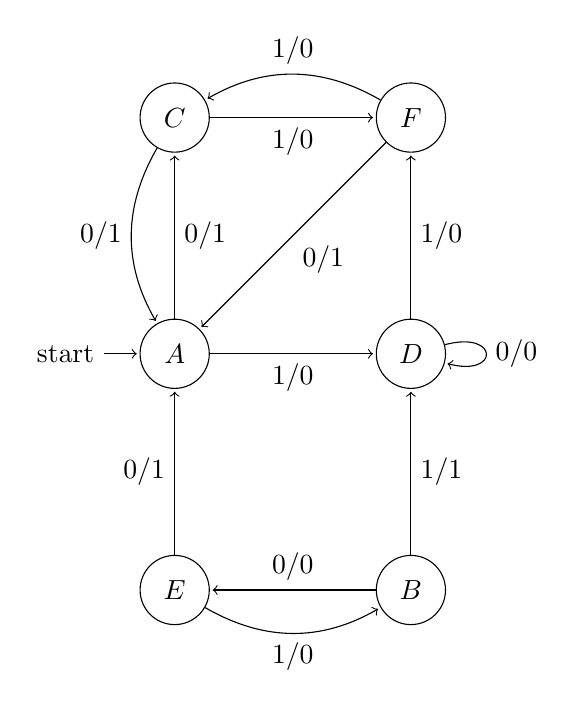
\begin{tikzpicture}[->,shorten >=1pt,node distance=3cm,on grid,auto]
					\node[state,initial] (A)                   {$A$};
					\node[state]		 (C) [above=of A]      {$C$};
					
					\node[state]		 (F) [right=of C]      {$F$};
					\node[state]		 (D) [below=of F] {$D$};
					\node[state]		 (B) [below=of D]       {$B$};
					\node[state]		 (E) [left=of B] {$E$};
					
					\path (A) edge              node [swap] {0/1} (C)
							  edge              node [swap] {1/0} (D)
						  (B) edge              node [swap] {0/0} (E)
							  edge              node [swap] {1/1} (D)
						  (C) edge [bend right] node [swap] {0/1} (A)
							  edge              node [swap] {1/0} (F)
						  (D) edge [loop right] node        {0/0} (D)
							  edge              node [swap] {1/0} (F)
						  (E) edge              node        {0/1} (A)
							  edge [bend right] node [swap] {1/0} (B)
						  (F) edge              node        {0/1} (A)
							  edge [bend right] node [swap] {1/0} (C);
				\end{tikzpicture}
			\end{center}
			
			\item A tree diagram representing (the accessible part of) the Mealy machine is shown in figure~\ref{fig:tree} below.
			\begin{figure}[H]
				\centering
				\begin{subfigure}[b]{0.45\textwidth}
					\centering
					\begin{tikzpicture}[
							->,
							shorten >=1pt,
							node distance=2.5cm,
							auto,
							level 1/.style={sibling distance=40mm},
							level 2/.style={sibling distance=20mm},
							level 3/.style={sibling distance=20mm}
						]
						\node {$A$}
							child {
								node {$C$}
								child {
									node {$A$}
								}
								child {
									node {$F$}
									child {
										node {$A$}
									}
									child {
										node {$C$}
									}
								}
							}
							child {
								node {$D$}
								child {
									node {$D$}
								}
								child {
									node {$F$}
								}
							}
						;
					\end{tikzpicture}
					\caption{}
					\label{fig:tree}
				\end{subfigure}
				\begin{subfigure}[b]{0.45\textwidth}
					\centering
					\begin{tabular}{r|C{6mm}|C{6mm}||C{6mm}|C{6mm}|}
						\cline{2-5}
						\multicolumn{1}{r|}{} &  \multicolumn{2}{c||}{Transition} & \multicolumn{2}{c|}{Output} \\
						\cline{2-5}
						& {\bf 0} & {\bf 1} & {\bf 0} & {\bf 1} \\
						\cline{2-5}
						 $\to A$ & $C$ & $D$ & 1 & 0 \\ \cline{2-5}
						 $C$	 & $A$ & $F$ & 1 & 0 \\ \cline{2-5}
						 $D$	 & $D$ & $F$ & 0 & 0 \\ \cline{2-5}
						 $F$	 & $A$ & $C$ & 1 & 0 \\
						\cline{2-5}
					\end{tabular}
					\caption{}
					\label{fig:table}
				\end{subfigure}
				\caption{}
			\end{figure}
			Notice that every "leaf state" was also included in the tree diagram as a "branch state." Thus, only the states shown in figure~\ref{fig:tree} are accessible. We therefore have the transition table in figure~\ref{fig:table}.
			
			\item The 0-equivalence classes are shown in the table below under the $\equiv _0$ column.
			\begin{center}
				\begin{tabular}{r|C{6mm}|C{6mm}||C{6mm}|C{6mm}|C{6mm}|}
					\cline{2-5}
					\multicolumn{1}{r|}{} &  \multicolumn{2}{c||}{Transition} & \multicolumn{2}{c|}{Output} & \multicolumn{1}{c}{} \\
					\cline{2-6}
					& {\bf 0} & {\bf 1} & {\bf 0} & {\bf 1} & $\equiv _0$ \\
					\cline{2-6}
					 $\to A$ & $C$ & $D$ & 1 & 0 & 0 \\ \cline{2-6}
					 $C$	 & $A$ & $F$ & 1 & 0 & 0 \\ \cline{2-6}
					 $D$	 & $D$ & $F$ & 0 & 0 & 1 \\ \cline{2-6}
					 $F$	 & $A$ & $C$ & 1 & 0 & 0 \\
					\cline{2-6}
				\end{tabular}
			\end{center}
			Although though this machine has only two 0-equivalence classes, there can be up to four. This is because the output set, whose cardinality is $2$, depends on the input set, whose cardinality is also $2$. (And $2 \times 2 = 4$.)
			
			\item The table showing equivalence classes is as follows.
			\begin{center}
				\begin{tabular}{r|C{6mm}|C{6mm}||C{6mm}|C{6mm}||C{5mm}|C{4mm}|C{4mm}||C{5mm}|C{4mm}|C{4mm}||C{5mm}|}
					\cline{2-5}
					\multicolumn{1}{r|}{} &  \multicolumn{2}{c||}{Transition} & \multicolumn{2}{c||}{Output} & \multicolumn{7}{c}{} \\ \cline{2-12}
					& {\bf 0} & {\bf 1} & {\bf 0} & {\bf 1} & $\equiv _0$ & {\bf 0} & {\bf 1} & $\equiv _1$ & {\bf 0} & {\bf 1} & $\equiv _2$ \\ \cline{2-12}
					 $\to A$ & $C$ & $D$ & 1 & 0 & 0 & 0 & 1 & 0 & 1 & 2 & 0 \\ \cline{2-12}
					 $C$	 & $A$ & $F$ & 1 & 0 & 0 & 0 & 0 & 1 & 0 & 1 & 1 \\ \cline{2-12}
					 $D$	 & $D$ & $F$ & 0 & 0 & 1 & 1 & 0 & 2 & 2 & 1 & 2 \\ \cline{2-12}
					 $F$	 & $A$ & $C$ & 1 & 0 & 0 & 0 & 0 & 1 & 0 & 1 & 1 \\ \cline{2-12}
				\end{tabular}
			\end{center}
			Identifying states $C$ and $F$ yields the Mealy machine shown below.
			\begin{center}
				\begin{tabular}{r|C{6mm}|C{6mm}||C{6mm}|C{6mm}|}
					\cline{2-5}
					\multicolumn{1}{r|}{} &  \multicolumn{2}{c||}{Transition} & \multicolumn{2}{c|}{Output} \\ \cline{2-5}
					& {\bf 0} & {\bf 1} & {\bf 0} & {\bf 1} \\ \cline{2-5}
					 $\to A$ & $C$ & $D$ & 1 & 0 \\ \cline{2-5}
					 $C$	 & $A$ & $C$ & 1 & 0 \\ \cline{2-5}
					 $D$	 & $D$ & $C$ & 0 & 0 \\ \cline{2-5}
				\end{tabular}
			\end{center}
			
			\item The reduced Mealy machine in standard form is as follows.
			\begin{center}
				\begin{tabular}{r|C{6mm}|C{6mm}||C{6mm}|C{6mm}|}
					\cline{2-5}
					\multicolumn{1}{r|}{} &  \multicolumn{2}{c||}{Transition} & \multicolumn{2}{c|}{Output} \\ \cline{2-5}
					& {\bf 0} & {\bf 1} & {\bf 0} & {\bf 1} \\ \cline{2-5}
					 $\to 0$ & $1$ & $2$ & 1 & 0 \\ \cline{2-5}
					 $1$	 & $0$ & $1$ & 1 & 0 \\ \cline{2-5}
					 $2$	 & $2$ & $1$ & 0 & 0 \\ \cline{2-5}
				\end{tabular}
			\end{center}
			
			\pagebreak
			
			\item Performing steps (d) and (e) on the given Mealy machine yields the following table of equivalence classes.
			\begin{center}
				\begin{tabular}{r|C{6mm}|C{6mm}||C{6mm}|C{6mm}||C{5mm}|C{4mm}|C{4mm}||C{5mm}|C{4mm}|C{4mm}||C{5mm}|}
					\cline{2-5}
					\multicolumn{1}{r|}{} &  \multicolumn{2}{c||}{Transition} & \multicolumn{2}{c||}{Output} & \multicolumn{7}{c}{} \\ \cline{2-12}
					& {\bf 0} & {\bf 1} & {\bf 0} & {\bf 1} & $\equiv _0$ & {\bf 0} & {\bf 1} & $\equiv _1$ & {\bf 0} & {\bf 1} & $\equiv _2$ \\ \cline{2-12}
					 $\to A$ & $C$ & $D$ & 1 & 0 & 0 & 0 & 2 & 0 & 2 & 3 & 0 \\ \cline{2-12}
					 $B$	 & $E$ & $D$ & 0 & 1 & 1 & 0 & 2 & 1 & 4 & 3 & 1 \\ \cline{2-12}
					 $C$	 & $A$ & $F$ & 1 & 0 & 0 & 0 & 0 & 2 & 0 & 2 & 2 \\ \cline{2-12}
					 $D$	 & $D$ & $F$ & 0 & 0 & 2 & 2 & 0 & 3 & 3 & 2 & 3 \\ \cline{2-12}
					 $E$	 & $A$ & $B$ & 1 & 0 & 0 & 0 & 1 & 4 & 0 & 1 & 4 \\ \cline{2-12}
					 $F$	 & $A$ & $C$ & 1 & 0 & 0 & 0 & 0 & 2 & 0 & 2 & 2 \\ \cline{2-12}
				\end{tabular}
			\end{center}
			Just as in part (e) of this question, states $C$ and $F$ can be identified. The inaccessible states were not however, as none of them were equivalent.
			
			In general, performing step (c) last will yield the same machine, however steps (d) and (e) are made more difficult.
			
			\item The Mealy machine can be converted to a Moore machine by having a version of each state for each possible output.
			
			For example, in the original machine, either a $0$ or a $1$ can be outputted in state $A$. In the corresponding Moore machine there should be one state $A_0$ which outputs a $0$ and another $A_1$ which outputs $1$. The resulting machine is shown below.
			\begin{center}
				\begin{tabular}{r|C{6mm}|C{6mm}||C{12mm}|}
					\multicolumn{1}{r}{} &  \multicolumn{2}{c}{Transition} & \multicolumn{1}{c}{Output} \\ \cline{2-3}
					& {\bf 0} & \multicolumn{1}{c||}{\bf 1} & \multicolumn{1}{c}{} \\ \cline{2-4}
					 $\to A_0$ & $C_1$ & $D_0$ & 0 \\ \cline{2-4}
					 $A_1$	 & $C_1$ & $D_0$ & 1 \\ \cline{2-4}
					 $B_0$	 & $E_0$ & $D_1$ & 0 \\ \cline{2-4}
					 $B_1$	 & $E_0$ & $D_1$ & 1 \\ \cline{2-4}
					 $C_0$	 & $A_1$ & $F_0$ & 0 \\ \cline{2-4}
					 $C_1$	 & $A_1$ & $F_0$ & 1 \\ \cline{2-4}
					 $D_0$	 & $D_0$ & $F_0$ & 0 \\ \cline{2-4}
					 $D_1$	 & $D_0$ & $F_0$ & 1 \\ \cline{2-4}
					 $E_0$	 & $A_1$ & $B_0$ & 0 \\ \cline{2-4}
					 $E_1$	 & $A_1$ & $B_0$ & 1 \\ \cline{2-4}
					 $F_0$	 & $A_1$ & $C_0$ & 0 \\ \cline{2-4}
					 $F_1$	 & $A_1$ & $C_0$ & 1 \\ \cline{2-4}
				\end{tabular}
			\end{center}
			Now we remove inaccessible states by creating a tree diagram of accesses.
			\begin{center}
				\begin{tikzpicture}[
						->,
						shorten >=1pt,
						node distance=2.5cm,
						auto,
						level 1/.style={sibling distance=80mm},
						level 2/.style={sibling distance=40mm},
						level 3/.style={sibling distance=20mm},
						level 4/.style={sibling distance=20mm}
					]
					\node {$A_0$}
						child {
							node {$C_1$}
							child {
								node {$A_1$}
								child {
									node {$C_1$}
								}
								child {
									node {$D_0$}
								}
							}
							child {
								node {$F_0$}
								child {
									node {$A_1$}
								}
								child {
									node {$C_0$}
									child {
										node {$A_1$}
									}
									child {
										node {$F_0$}
									}
								}
							}
						}
						child {
							node {$D_0$}
							child {
								node {$D_0$}
							}
							child {
								node {$F_0$}
							}
						}
					;
				\end{tikzpicture}
			\end{center}
			
			Preserving only the states shown in the above tree diagram (excluding the root) yields the following transition table.
			\begin{center}
				\begin{tabular}{r|C{6mm}|C{6mm}||C{12mm}|}
					\multicolumn{1}{r}{} &  \multicolumn{2}{c}{Transition} & \multicolumn{1}{c}{Output} \\ \cline{2-3}
					& {\bf 0} & \multicolumn{1}{c||}{\bf 1} & \multicolumn{1}{c}{} \\ \cline{2-4}
					 $\to A_1$	 & $C_1$ & $D_0$ & 1 \\ \cline{2-4}
					 $C_0$	 & $A_1$ & $F_0$ & 0 \\ \cline{2-4}
					 $C_1$	 & $A_1$ & $F_0$ & 1 \\ \cline{2-4}
					 $D_0$	 & $D_0$ & $F_0$ & 0 \\ \cline{2-4}
					 $F_0$	 & $A_1$ & $C_0$ & 0 \\ \cline{2-4}
				\end{tabular}
			\end{center}
			Creating a table to find equivalent states, we have the following.
			\begin{center}
				\begin{tabular}{r|C{5mm}|C{5mm}||C{5mm}|C{4mm}|C{4mm}||C{5mm}|C{4mm}|C{4mm}||C{5mm}|C{4mm}|C{4mm}||C{5mm}|}
					\cline{2-13}
					& {\bf 0} & {\bf 1} & $\equiv_0$ & {\bf 0} & {\bf 1} & $\equiv_1$ & {\bf 0} & {\bf 1} & $\equiv_2$ & {\bf 0} & {\bf 1} & $\equiv_3$ \\ \cline{2-13}
					 $\to A_1$	 & $C_1$ & $D_0$ & 1 & 1 & 0 & 0 & 0 & 2 & 0 & 2 & 3 & 0 \\ \cline{2-13}
					 $C_0$	 & $A_1$ & $F_0$ & 0 & 1 & 0 & 1 & 0 & 1 & 1 & 0 & 1 & 1 \\ \cline{2-13}
					 $C_1$	 & $A_1$ & $F_0$ & 1 & 1 & 0 & 0 & 0 & 1 & 2 & 0 & 1 & 2 \\ \cline{2-13}
					 $D_0$	 & $D_0$ & $F_0$ & 0 & 0 & 0 & 2 & 2 & 1 & 3 & 3 & 1 & 3 \\ \cline{2-13}
					 $F_0$	 & $A_1$ & $C_0$ & 0 & 1 & 0 & 1 & 0 & 1 & 1 & 0 & 1 & 1 \\ \cline{2-13}
				\end{tabular}
			\end{center}
			Identifying states $C_0$ and $F_0$ leaves us with the table shown below.
			\begin{center}
				\begin{tabular}{r|C{6mm}|C{6mm}||C{12mm}|}
					\multicolumn{1}{r}{} &  \multicolumn{2}{c}{Transition} & \multicolumn{1}{c}{Output} \\ \cline{2-3}
					& {\bf 0} & \multicolumn{1}{c||}{\bf 1} & \multicolumn{1}{c}{} \\ \cline{2-4}
					 $\to A_1$	 & $C_1$ & $D_0$ & 1 \\ \cline{2-4}
					 $C_0$	 & $A_1$ & $C_0$ & 0 \\ \cline{2-4}
					 $C_1$	 & $A_1$ & $C_0$ & 1 \\ \cline{2-4}
					 $D_0$	 & $D_0$ & $C_0$ & 0 \\ \cline{2-4}
				\end{tabular}
			\end{center}
			
			This Moore machine could have also been obtained by immediately converting from the reduced Mealy Machine in part (e).
			
			\item The reduced Moore machine is shown below in standard form.
			\begin{center}
				\begin{tabular}{r|C{6mm}|C{6mm}||C{12mm}|}
					\multicolumn{1}{r}{} &  \multicolumn{2}{c}{Transition} & \multicolumn{1}{c}{Output} \\ \cline{2-3}
					& {\bf 0} & \multicolumn{1}{c||}{\bf 1} & \multicolumn{1}{c}{} \\ \cline{2-4}
					 $\to 0$	 & 1 & 2 & 1 \\ \cline{2-4}
					 1	 & 0 & 3 & 1 \\ \cline{2-4}
					 2	 & 2 & 3 & 0 \\ \cline{2-4}
					 3	 & 0 & 3 & 0 \\ \cline{2-4}
				\end{tabular}
			\end{center}
		\end{enumerate}
		
		\item
		\begin{enumerate}
			\item From the tree diagram below, all states in the given FSA are accessible.
			\begin{center}
				\begin{tikzpicture}[
						->,
						shorten >=1pt,
						node distance=2.5cm,
						auto,
						level 1/.style={sibling distance=80mm},
						level 2/.style={sibling distance=40mm},
						level 3/.style={sibling distance=20mm},
						level 4/.style={sibling distance=20mm}
					]
					\node {$A$}
						child {
							node {$C$}
							child {
								node {$E$}
								child {
									node {$E$}
								}
								child {
									node {$C$}
								}
							}
							child {
								node {$D$}
								child {
									node {$A$}
								}
								child {
									node {$B$}
									child {
										node {$E$}
									}
									child {
										node {$C$}
									}
								}
							}
						}
						child {
							node {$F$}
							child {
								node {$C$}
								child {
									node {$E$}
								}
								child {
									node {$D$}
								}
							}
							child {
								node {$A$}
							}
						}
					;
				\end{tikzpicture}
			\end{center}
			
			\item To reduce a finite state machine, inaccessible states (if they exist) must be removed.
			
			\pagebreak
			
			\item The table showing equivalence classes for the given FSA is included below.
			\begin{center}
				\begin{tabular}{r|C{5mm}|C{5mm}||C{5mm}|C{4mm}|C{4mm}||C{5mm}|C{4mm}|C{4mm}||C{5mm}|C{4mm}|C{4mm}||C{5mm}|C{4mm}|C{4mm}||C{5mm}|}
					\cline{2-16}
					& {\bf 0} & {\bf 1} & $\equiv_0$ & {\bf 0} & {\bf 1} & $\equiv_1$ & {\bf 0} & {\bf 1} & $\equiv_2$ & {\bf 0} & {\bf 1} & $\equiv_3$ & {\bf 0} & {\bf 1} & $\equiv_4$ \\ \cline{2-16}
					$\to A$	 & $C$ & $F$ & 0 & 1 & 0 & 0 & 1 & 0 & 0 & 1 & 0 & 0 & 2 & 0 & 0 \\ \cline{2-16}
					$B$	 	 & $E$ & $C$ & 1 & 0 & 1 & 1 & 2 & 1 & 1 & 3 & 1 & 1 & 4 & 2 & 1 \\ \cline{2-16}
					$C$	 	 & $E$ & $D$ & 1 & 0 & 1 & 1 & 2 & 1 & 1 & 3 & 2 & 2 & 4 & 3 & 2 \\ \cline{2-16}
					$D$	 	 & $A$ & $B$ & 1 & 0 & 1 & 1 & 0 & 1 & 2 & 0 & 1 & 3 & 0 & 1 & 3 \\ \cline{2-16}
					$E$	 	 & $E$ & $C$ & 0 & 0 & 1 & 2 & 2 & 1 & 3 & 3 & 1 & 4 & 4 & 2 & 4 \\ \cline{2-16}
					$F$	 	 & $C$ & $A$ & 0 & 1 & 0 & 0 & 1 & 0 & 0 & 1 & 0 & 0 & 2 & 0 & 0 \\ \cline{2-16}
				\end{tabular}
			\end{center}
			From the table, states $A$ and $F$ are equivalent. This is shown in the state diagram which follows.
			\begin{center}
				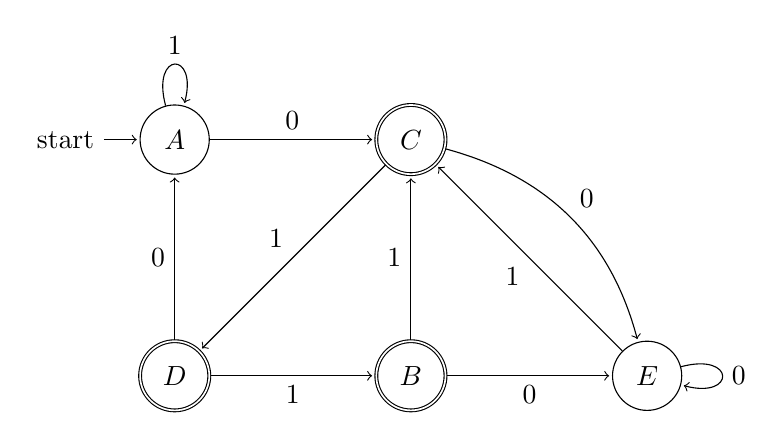
\begin{tikzpicture}[->,shorten >=1pt,node distance=3cm,on grid,auto]
					\node[state,initial]   (A)                   {$A$};
					\node[state,accepting] (C) [right=of A] {$C$};
					\node[state,accepting] (D) [below=of A] {$D$};
					\node[state,accepting] (B) [below=of C] {$B$};
					\node[state]           (E) [right=of B] {$E$};
					
					\path (A) edge              node        {0} (C)
							  edge [loop above] node        {1} (A)
						  (B) edge              node [swap] {0} (E)
							  edge              node        {1} (C)
						  (C) edge [bend left]  node        {0} (E)
							  edge              node [swap] {1} (D)
						  (D) edge              node        {0} (A)
							  edge              node [swap] {1} (B)
						  (E) edge [loop right] node        {0} (E)
							  edge              node        {1} (C);
				\end{tikzpicture}
			\end{center}
			
			\item The reduced FSA can be also be written as a transition table.
			\begin{center}
				\begin{tabular}{r|C{5mm}|C{5mm}|l}
					\cline{2-3}
					& {\bf 0} & {\bf 1} & \\ \cline{2-3}
					$\to A$	 & $C$ & $A$ &        \\ \cline{2-3}
					$B$	 	 & $E$ & $C$ & $\ast$ \\ \cline{2-3}
					$C$	 	 & $E$ & $D$ & $\ast$ \\ \cline{2-3}
					$D$	 	 & $A$ & $B$ & $\ast$ \\ \cline{2-3}
					$E$	 	 & $E$ & $C$ &        \\ \cline{2-3}
				\end{tabular}
			\end{center}
			
			\item In standard form, the machine is as follows.
			\begin{center}
				\begin{tabular}{r|C{5mm}|C{5mm}|l}
					\cline{2-3}
					& {\bf 0} & {\bf 1} & \\ \cline{2-3}
					$\to 0$	 & 1 & 0 &        \\ \cline{2-3}
					1	 	 & 2 & 3 & $\ast$ \\ \cline{2-3}
					2	 	 & 2 & 1 &        \\ \cline{2-3}
					3	 	 & 0 & 4 & $\ast$ \\ \cline{2-3}
					4	 	 & 2 & 1 & $\ast$ \\ \cline{2-3}
				\end{tabular}
			\end{center}
		\end{enumerate}
	\end{enumerate}
\end{document}
